\documentclass{beamer}

\usepackage{math214}

\usepackage{hyperref}
\usepackage{caption}
\DeclareCaptionLabelFormat{black}{\textcolor{black}{#1~#2}}
\captionsetup[figure]{labelformat=black}
\captionsetup[figure]{font=tiny}
\usepackage{listings}
\usepackage[linesnumbered,ruled]{algorithm2e}


\title{Gradient Descent in Machine Learning}
\author{pgroup1}
\date{Spring 2023}

% \definecolor{darkblue}{HTML}{6666dd} 
% \colortheme{green!42!black}
% \colortheme{orange!85!black}
% \colortheme{darkblue}
% \colortheme{pink!80!black}
\colortheme{orange!85!white!90!black}

\begin{document}

\maketitle




%%%%%%%%%%%%%%%%%%%%%%%%%%%%%%%%%%%%%%%%%%%%%%%%%%%%%%%%%%%%%%%%%%%
\section{The basic principle}

\begin{frame}{The basic principle}

Motivation:Want machines to make more accurate predictions after fed with training sets.

Outline of gradient descent algorithms:
\begin{center}
 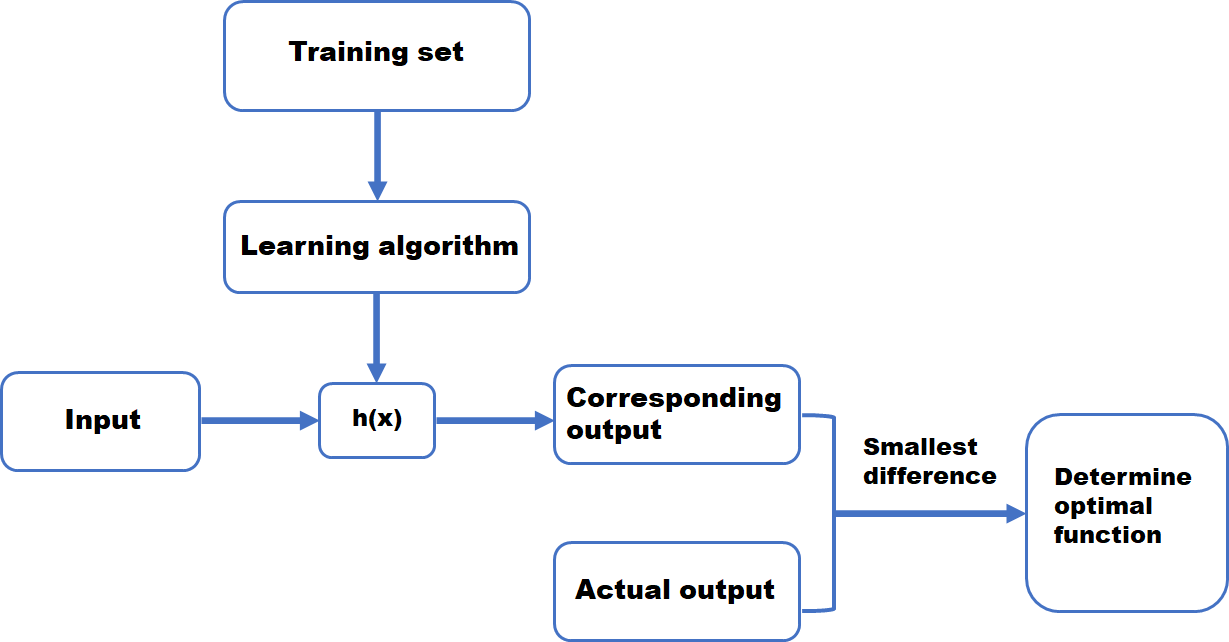
\includegraphics[width=.9\columnwidth]{img/outline.PNG}
\end{center}
\end{frame}
\begin{frame}{Hypothesis function}
Why linear regression?
\begin{itemize}
    \item Simple and proper way to get the information from training set
    \item Related to the linear algebra
\end{itemize}
\begin{theorem}

                        Hypothesis function:
  
         $$h_{\theta}(x):=\theta_0+\sum_{i=1}^{m}(\theta_i x_i)$$
         x represents several elements that affect final result,\\
         and theta represents corresponding weight of each element.



\end{theorem}
\end{frame}
\begin{frame}{Loss function}
Target:Want to make prediction more accurate.\\
Mathematical understanding:Make the difference between predicted value and actual one as small as possible.\\
Method:Use a special function to achieve it.\\
So,we introduce a new function,
\begin{theorem}
Loss function:


        $$J(\theta_0,\theta_1...,\theta_m):=\frac{1}{2n}\sum_{j=1}^{n}((h_{\theta}(x_0^{(j)},x_1^{(j)},x_m^{(j)})-y^{(j)})^{2}$$
 n equals to the size of training set.
\end{theorem}
\end{frame}
\begin{frame}{The basic principle}
Some properties of loss function:(under the case of linear regression)\\
\begin{itemize}
    \item convexity
\end{itemize}
One-parameter figure:\\
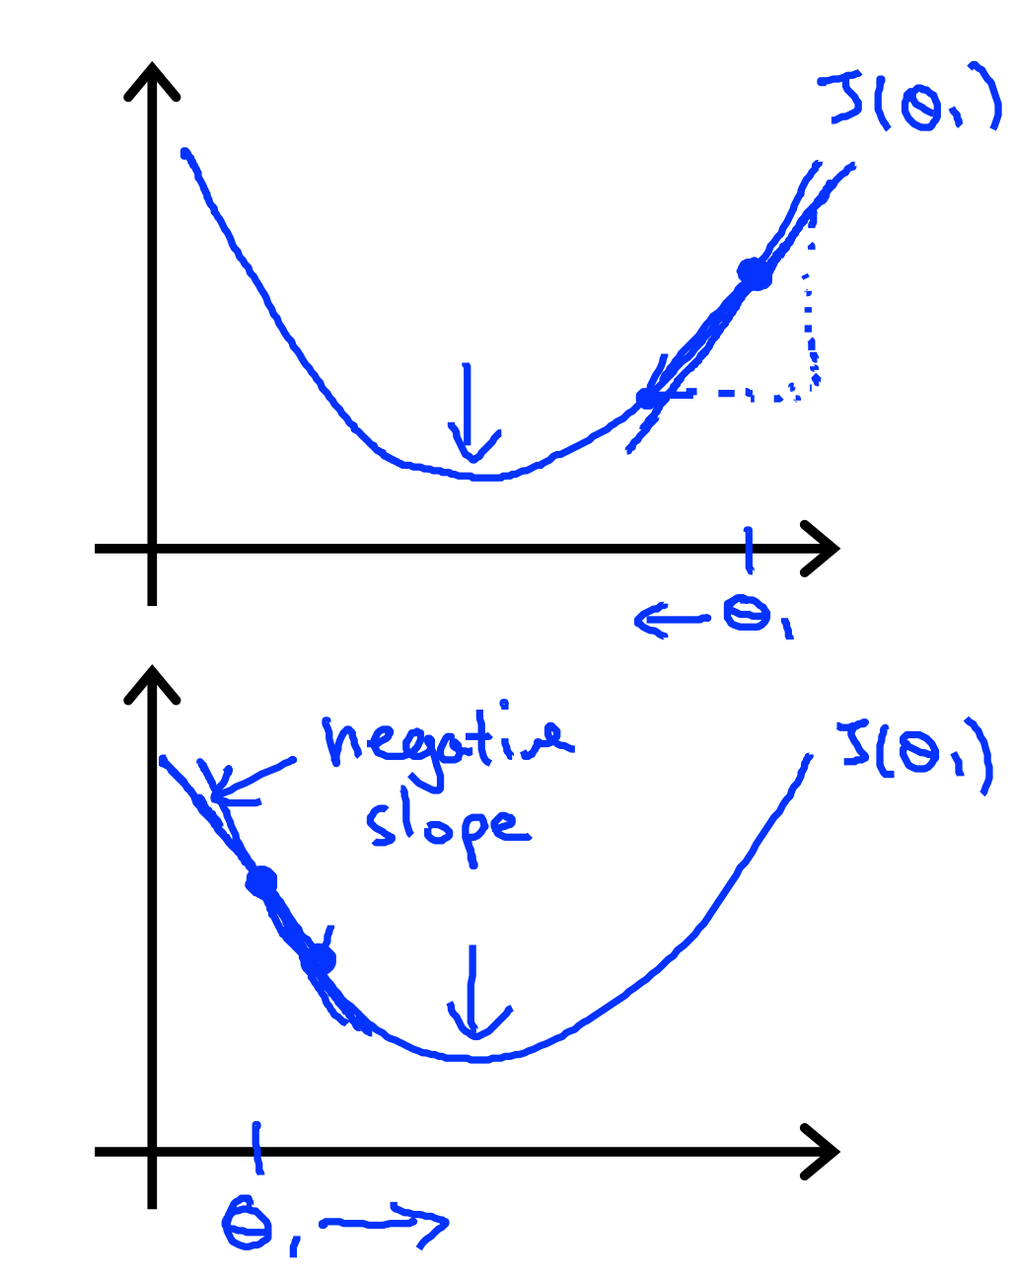
\includegraphics[width=.5\columnwidth]{img/graph1.PNG}
\end{frame}
\begin{frame}{Convexity}
Two-parameters figure:
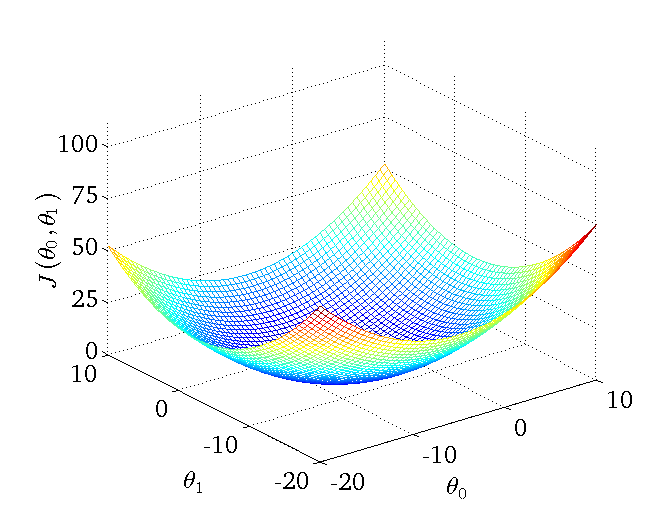
\includegraphics[width=.7\columnwidth]{img/graph2.PNG}
\end{frame}
\begin{frame}{Convexity}
Convexity guarantees that we can find the global minimum.\\
\begin{theorem}

For $\theta_j$,
                    $$ \theta_j \leftarrow \theta_j-\alpha \frac{d}{d\theta_i}J(\theta_0,\theta_1,...\theta_m)$$
alpha represents the learning efficiency.
\end{theorem}
After calculation, we find that,
when j equals to 0,\\
$$\frac{d}{d\theta_j}J(\theta_0,\theta_1,...\theta_m)=\frac{1}{n}\sum_{i=1}^{n}(h_{\theta}(x_0^{(i)},x_1^{(i)},...x_m^{(i)})-y^{(i)}),$$
when j is an integer larger than 0,\\
$$\frac{d}{d\theta_j}J(\theta_0,\theta_1,...\theta_m)=\frac{1}{n}\sum_{i=1}^{n}(h_{\theta}(x_0^{(i)},x_1^{(i)},...x_m^{(i)})-y^{(i)})x_j^{(i)},$$
repeat until convergence.


\end{frame}
\begin{frame}{Vectorizing Gradient Descent}
Why vectorizing?
\begin{itemize}
    \item Simpler notations.
    \item Faster training speed in programming.
\end{itemize}

$$
X = \begin{bmatrix}
    x^{(1)}\\x^{(2)}\\\vdots\\x^{(n)}
\end{bmatrix}
=
\begin{bmatrix}
    x_0^{(1)}&x_1^{(1)}&\cdots&x_m^{(1)}\\
    x_0^{(2)}&x_1^{(2)}&\cdots&x_m^{(2)}\\
    \vdots&\vdots&\ddots&\vdots\\
    x_0^{(n)}&x_1^{(n)}&\cdots&x_m^{(n)}\\
\end{bmatrix},
y = \begin{bmatrix}
    y^{(1)}\\y^{(2)}\\\vdots\\y^{(n)}
\end{bmatrix},
\theta = \begin{bmatrix}
    \theta^{(1)}\\\theta^{(2)}\\\vdots\\\theta^{(m)}
\end{bmatrix}
$$
$$
\begin{aligned}
\theta_j &:= \theta_j - \alpha \sum_{i=1}^{n}(h_{\theta}(x^{(i)})-y^{(i)})x_j^{(i)}\\
&= \theta_0 - \alpha \begin{bmatrix}
x_j^{(1)}&x_j^{(2)}&\cdots&x_j^{(n)}\\
\end{bmatrix}
(h_{\theta}(x)-y)\\
&= \theta_0 - \alpha \begin{bmatrix}
x_j^{(1)}&x_j^{(2)}&\cdots&x_j^{(n)}\\
\end{bmatrix}
(x\cdot\theta-y)\\
\end{aligned}
$$
\end{frame}

\begin{frame}{Vectorizing Gradient Descent}
Synthesizing all $j \in [i,n]$,
$$
\begin{bmatrix}
    \theta^{(1)}\\\theta^{(2)}\\\vdots\\\theta^{(m)}
\end{bmatrix}
:=
\begin{bmatrix}
    \theta^{(1)}\\\theta^{(2)}\\\vdots\\\theta^{(m)}
\end{bmatrix}
- \alpha
\begin{bmatrix}
    x_0^{(1)}&x_0^{(1)}&\cdots&x_0^{(n)}\\
    x_1^{(1)}&x_1^{(1)}&\cdots&x_1^{(n)}\\
    \vdots&\vdots&\ddots&\vdots\\
    x_m^{(1)}&x_m^{(2)}&\cdots&x_m^{(n)}\\
\end{bmatrix}
(X\cdot\theta - y)
$$

\begin{theorem}
    Vectorized form of gradient descent in linear regression.
    
    $$\theta := \theta - \alpha X^{\top}(X\theta - y)$$
\end{theorem}
    
\end{frame}


%%%%%%%%%%%%%%%%%%%%%%%%%%%%%%%%%%%%%%%%%%%%%%%%%%%%%%%%%%%%%%%%%%%
\section{Application of Gradient Descent: MNIST}
\begin{frame}{Application Introduction}
	\begin{columns}[T,onlytextwidth]
		\column{.4\textwidth}
		\begin{figure}
			\centering 
			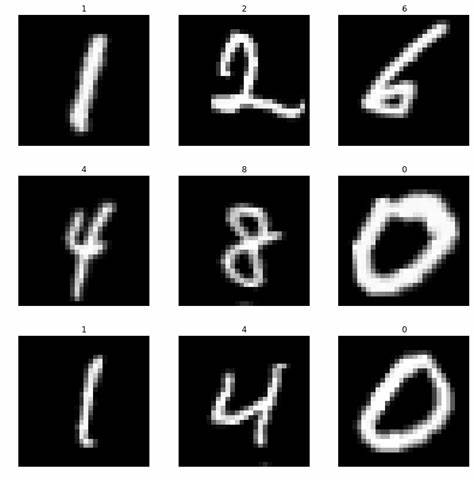
\includegraphics[width=1\columnwidth,height=6cm]{img/mnist.jpg}
			\caption{}
		\end{figure}
	
		\column{.6\textwidth}
		\begin{itemize}
			\item MNIST is a famous dataset used for image
			recognition and classification tasks. It consists 
			of 70,000 (60,000 training+10,000 testing) 
			handwritten digits in a 28x28 px grayscale image.
			\item Our project application is to use CNN model
			predict MNIST handwritten digits. In the application,
			we discover how Gradient Descent applies in DL.
			\item Project source code repo: \href{https://github.com/openhe-hub/math214-project.git}{https://github.com/openhe-hub/math214-project.git} 
		\end{itemize}
	\end{columns}	
\end{frame}

\begin{frame}{Model Introduction}
	\begin{columns}[T,onlytextwidth]
		\column{.4\textwidth}
		\begin{figure}
			\centering 
			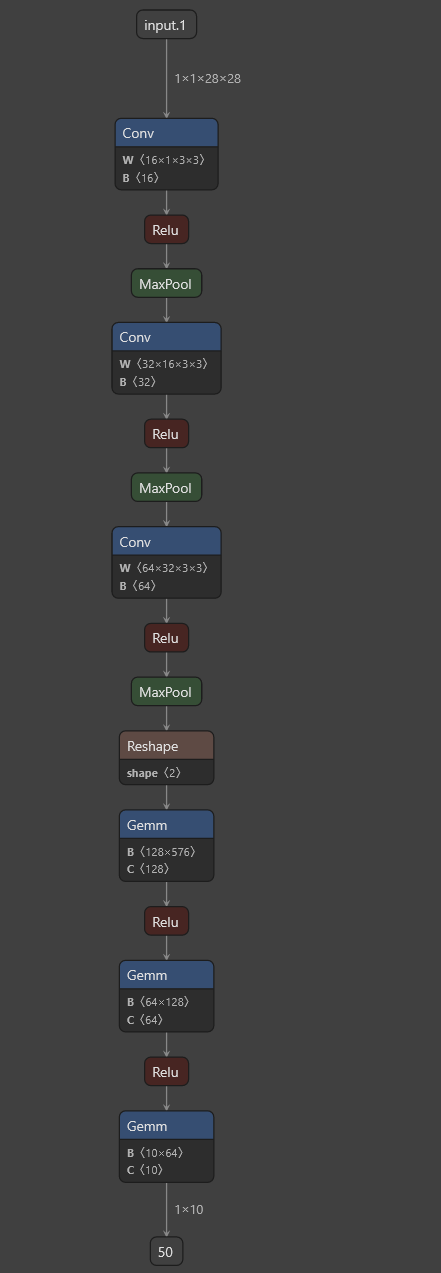
\includegraphics[width=0.85\columnwidth, height=7.5cm]{img/model.png}
			\caption{CNN Model (visualized by Netron)}
		\end{figure}

		\column{.6\textwidth}
		\begin{itemize}
			\item Our CNN Model: \newline 3 $conv\_layers$ (Conv+Relu+MaxPool)\newline+1 $fc\_layer$ (Linear+Relu)
			\item Loss function: $CrossEntropy$
			\item Gradient Descent: $SGD$
			\item Other Parameters: 
				\begin{itemize}
					\item $epochs=30$
					\item $batch\_size=64$
					\item $learning\_rate=0.001$
				\end{itemize}
		\end{itemize}
	\end{columns}
\end{frame}


\begin{frame}{Gradient Descent}
	\begin{theorem}
		SGD Iteration Formula: $w_{t+1} = w_t - \eta \nabla L(w_t)$
	\end{theorem}
	\begin{algorithm}[H]
		\SetAlgoLined
		\KwData{Input data $x$ and labels $y$}
		\KwResult{Trained CNN model}
		\SetKwFunction{FMain}{Train}
		\SetKwProg{Fn}{Function}{:}{}
		\Fn{\FMain{}}{
			\For{$epoch$ =1 to $epochs$}{
				\For{$batch\_i=(x_i,y_i)$ in $dataset$}{
					Set gradients of network parameters to zero\;
					Forward propagation: $\hat{y}$=forward($x_i$)\;
					Compute loss function: $loss$=$L(\hat{y}, y_i)$\;
					Backward propagation: $loss$.backward()\;
					Update parameters using SGD: $w = w - \eta \nabla L(w)$\;
				}
			}
		}
		\caption{SGD algorithm for training a CNN}
	\end{algorithm}
\end{frame}

\begin{frame}{Conclusion}
	\begin{columns}[T,onlytextwidth]
		\column{.45\textwidth}
		\begin{figure}
			\centering 
			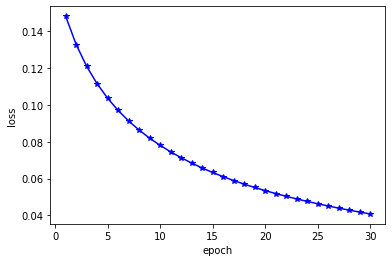
\includegraphics[width=1\columnwidth,height=4.2cm]{img/loss.png}
			\caption{SGD epoch-loss plot}
		\end{figure}

		\column{.05\textwidth}
	
		\column{.5\textwidth}
		  \quad The epoch-loss plot  shows how the model's 
		  loss function changes over time, as it updates the model 
		  parameters using small batches of training data. The plot 
		  typically displays a downward trend, with rapid 
		  loss reductions in initial epochs, and slower reductions 
		  as the algorithm converges. 
	\end{columns}
\end{frame}

\begin{frame}{Classification Result}
	\begin{columns}[T,onlytextwidth]
		\column{.45\textwidth}
		\begin{figure}
			\centering 
			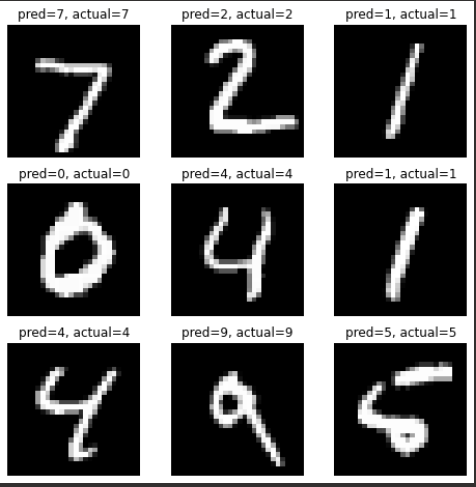
\includegraphics[width=1\columnwidth,height=5.5cm]{img/result.png}
			\caption{Testing set prediction result}
		\end{figure}

		\column{.05\textwidth}
	
		\column{.5\textwidth}
		\begin{itemize}
			\item Result: The total loss is about $0.0413$, 
			and the accuracy is about $98.67\%$. Algorithms (SGD) 
			based on Gradient Descent works well in our CNN model.
			\item Improvement: Consider adjusting
			parameters like $learning\_rate$, $batch\_size$. Also, we may 
			change different GD algorithms like $Adam$.
		\end{itemize} 
	\end{columns}
\end{frame}

%%%%%%%%%%%%%%%%%%%%%%%%%%%%%%%%%%%%%%%%%%%%%%%%%%%%%%%%%%%%%%%%%%%
\section{Improved Gradient Descents}
%%%%%%%%%%%%%%%%%%%
\begin{frame}{Improved Gradient Descents}

Motivation: Wants to improve learning efficiency (always!), reduce fluctuation, avoid local minima, etc.

Improved gradient descent algorithms:
\begin{center}
    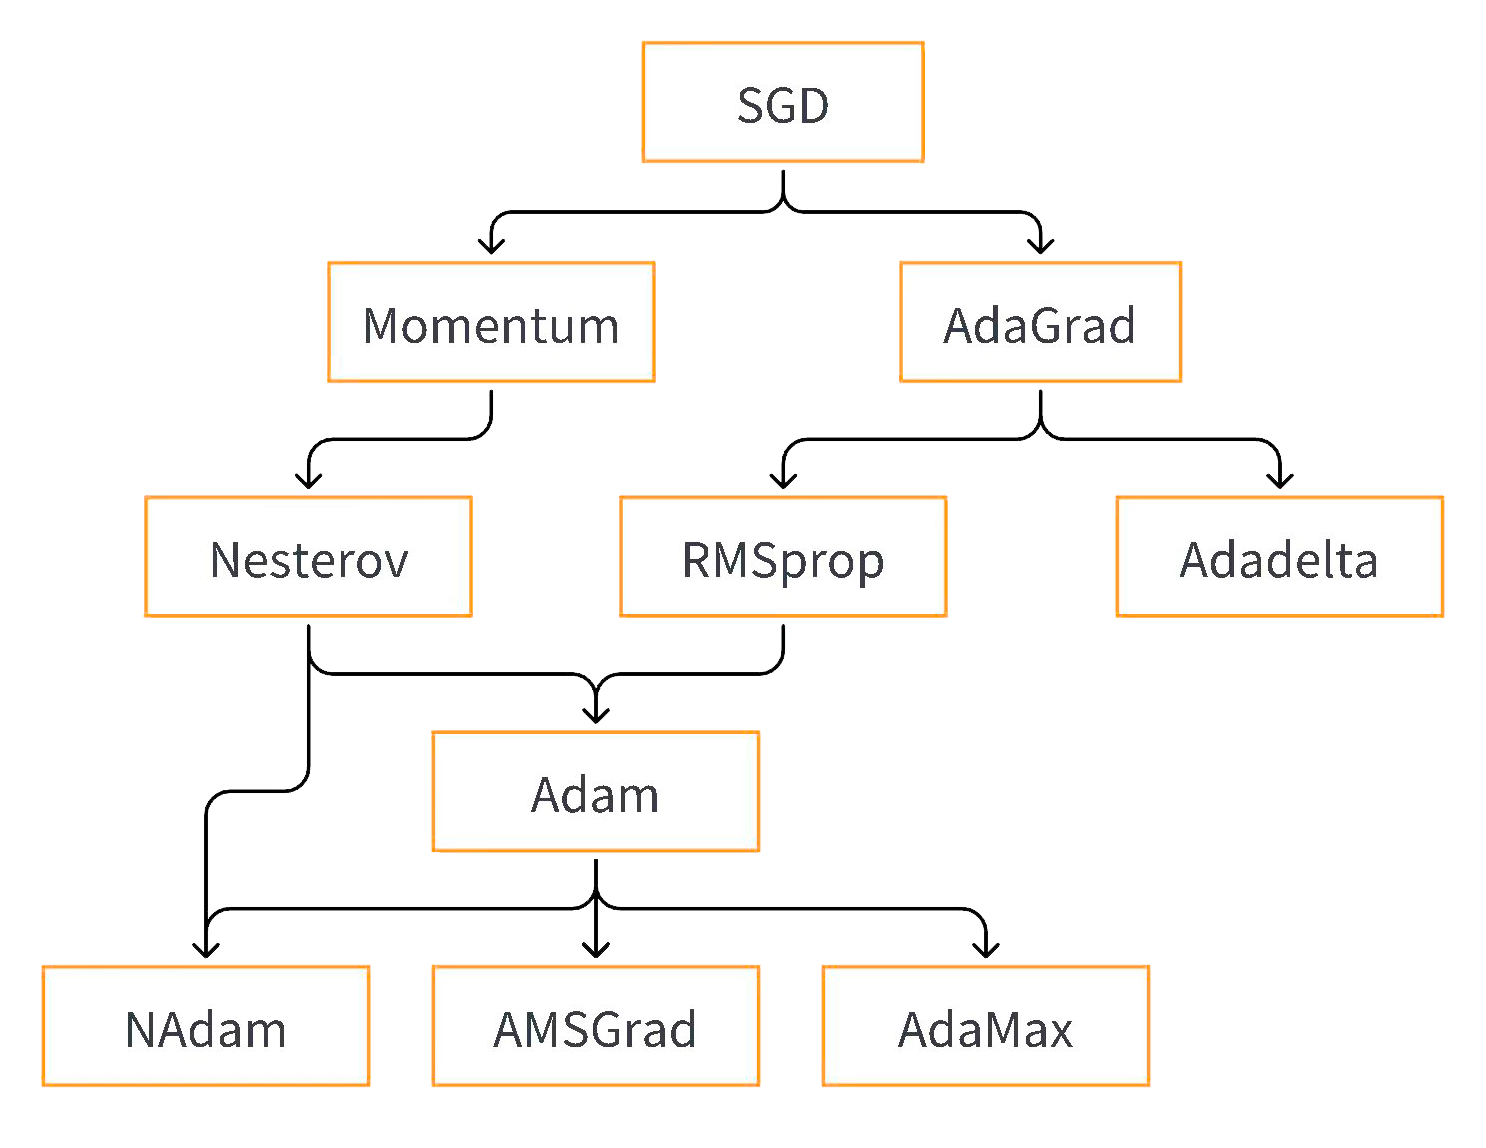
\includegraphics[width=.7\columnwidth]{img/improve.png}
\end{center}
\end{frame}
%%%%%%%%%%%%%%%%%%%
\begin{frame}{Gradient Descent with momentum}
\begin{theorem}
    For $\theta_j$,
    $$v_j \leftarrow \eta v_j - \alpha \nabla_{\theta_j}J(\theta)$$
    $$\theta_j \leftarrow \theta_j - v_j$$
\end{theorem}

Illustration: Keep accumulating momentum (velocity) when rolling down a slope.

\begin{columns}[T,onlytextwidth]

	\column{.33\textwidth}
	\centering 
	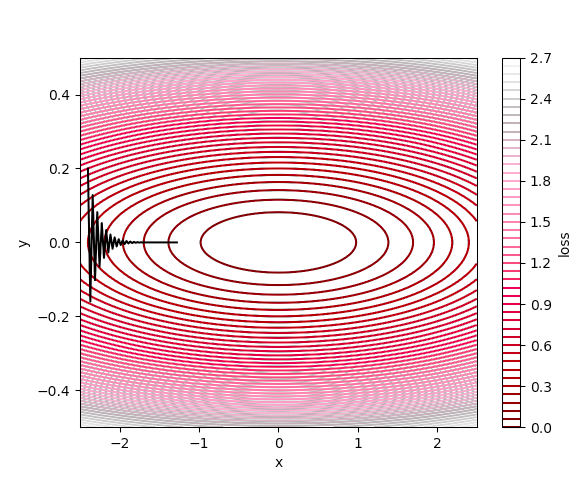
\includegraphics[width=1\columnwidth]{img/momentum0.png}
    $\eta = 0$
    
	\column{.33\textwidth}
	\centering 
	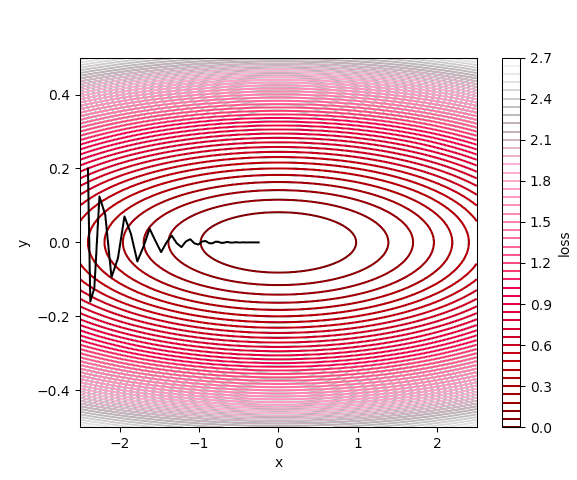
\includegraphics[width=1\columnwidth]{img/momentum07.png}
	$\eta = 0.7$
	
	\column{.33\textwidth}
	\centering 
	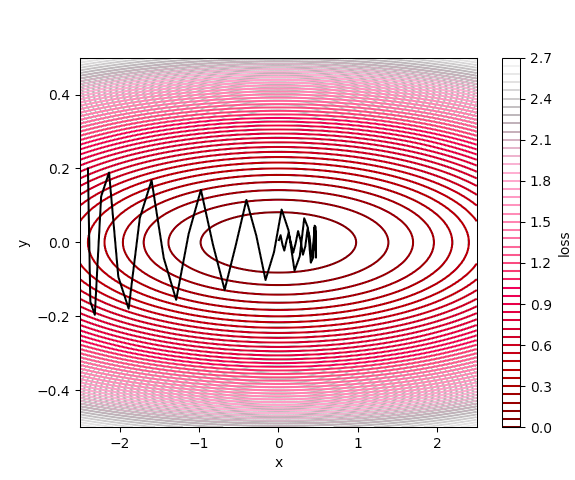
\includegraphics[width=1\columnwidth]{img/momentum09.png}
	$\eta = 0.9$

\end{columns}


\end{frame}
%%%%%%%%%%%%%%%%%%%
\begin{frame}{Gradient Descent with momentum}


\begin{center}
    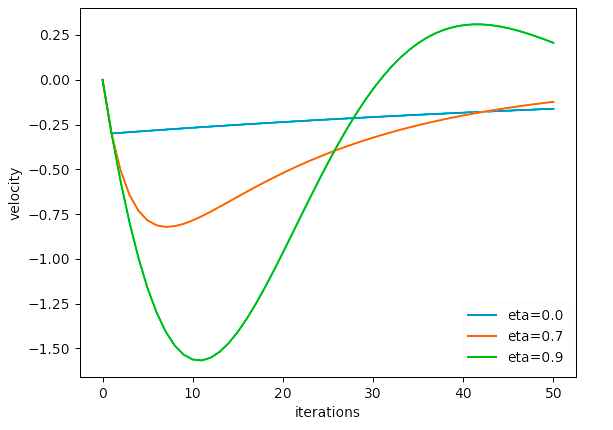
\includegraphics[width=.6\columnwidth]{img/velocity_momentum.png}
    \\
    Descent velocity comparison.
\end{center}
Advantages of GD with momentum:
\begin{enumerate}
    \item Accelerate the correct direction, and decelerate the wrong direction.
    \item Reduce fluctuation in the ``valley area".
\end{enumerate}



\end{frame}

%%%%%%%%%%%%%%%%%%%
% \begin{frame}{Nesterov accelerated gradient}
% \begin{theorem}
%     For $\theta_j$,
%     $$v_j \leftarrow \eta v_j - \alpha \nabla_{\theta_j}J(\theta - \eta v_j)$$
%     $$\theta_j \leftarrow \theta_j - v_j$$
% \end{theorem}

% Illustration:
% \begin{itemize}
%     \item Make predictions of the future gradient.
%     \item A more layer of acceleration.
% \end{itemize}

% \end{frame}













\begin{frame}{AdaGrad}
\begin{theorem}
    For $\theta_j$,
    $$ g_{t,j} = \nabla_{\theta_{t,j}}J(\theta) $$
    $$ G_{t,j} = G_{t-1,j} + g_{t,j}^2  $$
    $$\theta_{t+1,j} = \theta_{t,j} - \frac{\alpha}{\sqrt{G_{t,j} + \epsilon}} g_{t,j}$$
    
\end{theorem}
Illustration:
\begin{itemize}
    \item Automatically adapt the learning rate to the gradient.
\end{itemize}

\begin{columns}[T,onlytextwidth]

	\column{.33\textwidth}
	\centering 
	\includegraphics[width=1\columnwidth, height=0.65\columnwidth]{img/comparison of GD/local min/localGD.png}
    gradient descent
    
	\column{.33\textwidth}
	\centering 
	\includegraphics[width=1\columnwidth, height=0.65\columnwidth]{img/comparison of GD/local min/localMom.png}
	momentum
	
	\column{.33\textwidth}
	\centering 
	\includegraphics[width=1\columnwidth, height=0.65\columnwidth]{img/comparison of GD/local min/localADA.png}
	adagrad

\end{columns}







\end{frame}

\begin{frame}{Comparison in Saddle}

\begin{center}
	\includegraphics[width=0.6\columnwidth]{img/comparison of GD/saddle/saddle.png}
    \\
    Gradient Descent in Saddle.
\end{center}
Advantages of AdaGrad:
\begin{enumerate}
    \item Eliminate fluctuation.
    \item Decrease reliably.

\end{enumerate}




\end{frame}



\begin{frame}{Comparison in Plateau}

\begin{center}
	\includegraphics[width=0.6\columnwidth]{img/comparison of GD/plateau/plateau.png}
    \\
    Gradient Descent in Plateau.
\end{center}
Disadvantages of AdaGrad:
\begin{enumerate}
    \item Decrease slow if gradients are high.
    \item Stuck in ``valleys" or ``plateaux".
\end{enumerate}


\end{frame}









\begin{frame}{Matrix Implementation}
\begin{theorem}
    $$ g_{t} = \nabla_{\theta}J(\theta) = 
    \begin{bmatrix} 
        \nabla_{\theta_{t,1}}J(\theta) \\ 
        \nabla_{\theta_{t,2}}J(\theta) \\
        \vdots \\
        \nabla_{\theta_{t,n}}J(\theta) 
        
\end{bmatrix}$$
    $$ G_{t} = \sum_{\tau=1}^t g_{\tau}g_{\tau} ^T = \sum_{\tau=1}^t
    \begin{bmatrix} 
        \nabla_{\theta_{\tau,1}}^2J(\theta) & \ast & \cdots & \ast\\ 
        \ast & \nabla_{\theta_{\tau,2}}^2J(\theta) & \cdots & \ast\\
        \vdots & \vdots & \ddots & \vdots \\ 
        \ast & \ast & \cdots & \nabla_{\theta_{\tau,n}}^2J(\theta) \\ 
    \end{bmatrix}$$
    
    $$\theta_{t+1} = \theta_{t} - \alpha  (diag(G_t) +\epsilon I_n)^{-\frac{1}{2}}  g_{t}$$
    
\end{theorem}

\end{frame}

\begin{frame}{Matrix Implementation}
\begin{theorem}

 
%  $$ \theta_{t+1} = \theta_{t} - \alpha  (diag(G_t) +\epsilon I_n)^{-\frac{1}{2}}  g_{t}$$
  
% $$
%  \begin{bmatrix} 
%         \theta_{t+1,1} \\ 
%         \theta_{t+1,2}  \\
%         \vdots\\
%         \theta_{t+1,n}  
% \end{bmatrix} = \begin{bmatrix} 
%     \theta_{t,1} \\ 
%     \theta_{t,2}  \\
%     \vdots\\
%     \theta_{t,n}  
% \end{bmatrix}
% - \alpha 
%     \begin{bmatrix} 
%         G_{t,1} +\epsilon & 0 & \cdots & 0\\ 
%         0 & G_{t,2}+\epsilon & \cdots & 0\\
%         \vdots & \vdots & \ddots & \vdots \\ 
%         0 & 0 & \cdots & G_{t,n}+\epsilon 
%     \end{bmatrix}^{-\frac{1}{2}}
%     \begin{bmatrix} 
%     g_{t,1} \\ 
%     g_{t,2}  \\
%     \vdots\\
%     g_{t,n} 
% \end{bmatrix}\\
%  \begin{bmatrix} 
%         \theta_{t+1,1} \\ 
%         \theta_{t+1,2}  \\
%         \vdots\\
%         \theta_{t+1,n}  
% \end{bmatrix}  
% =     \begin{bmatrix} 
%     \theta_{t,1} \\ 
%     \theta_{t,2}  \\
%     \vdots\\
%     \theta_{t,n}  
% \end{bmatrix}
% - 
%     \begin{bmatrix} 
%       \frac{\alpha}{\sqrt{ G_{t,1} +\epsilon }}& 0 & \cdots & 0\\ 
%         0 & \frac{\alpha}{\sqrt{ G_{t,2} +\epsilon }} & \cdots & 0\\
%         \vdots & \vdots & \ddots & \vdots \\ 
%         0 & 0 & \cdots &\frac{\alpha}{\sqrt{ G_{t,n} +\epsilon }}
%     \end{bmatrix}
%     \begin{bmatrix} 
%     g_{t,1} \\ 
%     g_{t,2}  \\
%     \vdots\\
%     g_{t,n}  
% \end{bmatrix}
% $$


\end{theorem}

\end{frame}






% %%%%%%%%%%%%%%%%%%%
% \begin{frame}{Python Implementation}
% Code of GD with momentum:
% \begin{center}
%     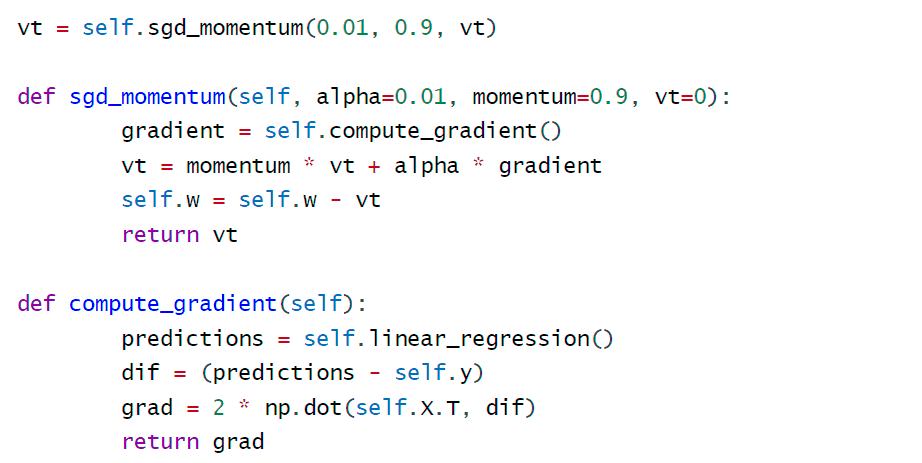
\includegraphics[width=.9\columnwidth]{gdmcode.png}
% \end{center}

% Code of Nesterov accelerated gradient:
% \begin{center}
%     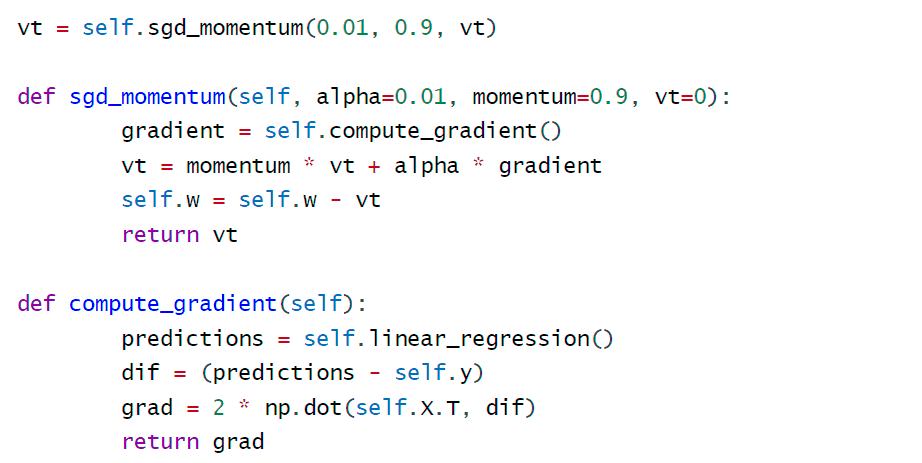
\includegraphics[width=.9\columnwidth]{gdmcode.png}
% \end{center}
% \end{frame}

\thankframe

\end{document}
